\documentclass{article}

\usepackage{fullpage}
\usepackage{graphicx}

\begin{document}

\title{Approximating Functions for Grid Domains}
\author{Danny Zhu (dannyz) \and Yuzi Nakamura (ynakamur) \and Ben Humberston (bhumbers)}

\maketitle

\section{Introduction}

Approximate computing is a method of computation that sacrifices accuracy for computation time and energy. For certain problems, a large degree of precision may not be necessary, and the savings gained in battery life or power costs may be worth more than the accuracy lost. In particular, we are inspired by the RoboCup code, where speed in decision-making trades off with the optimality of the final decision. Approximate compilation is a promising way of implementing approximate computation that can be done on current machines.

In this project, we take several C functions and compile them into various approximators (also C functions, with the same function signature). We then analyze them to determine the speedup and how well they approximate the original.

\section{Related Work}
In tandem with the renewed focus on paralell computing, interest in general purpose approximate computing increased recently in response to the decelerating efficiency gains for traditional scalar microprocessors. Techniques in approximate compilation automatically produce inexact yet more efficient versions of programmer-specified ``approximable'' code regions or data structures. An approximating compiler is thus responsible for encapsulating the low-level implementation of approximated code derived, typically, from high level source. The programmer's input over how the approximation is implemented may only be binary (eg: annotating some functions as ``approximable'', as in \cite{Esmaeilzadeh12}), or they may be given finer-grained control over the tradeoff between accuracy and speedup of the approximation, as in the quality programmable machine instructions from \cite{Venkataramani13}.

\cite{Agarwal09} introduces the SpeedPress compiler and SpeedGuard runtime which make use of an approximate compilation strategy that they term ``code perforation''. This strategy selectively drops iterations from long-lasting loops based on the current value of a user-defined quality metric. It has the advantage of allowing a computation to be dynamically retargeted for either realtime performance or accuracy, a useful property for time-critical systems.

Although our project is restricted to software approximation schemes, our primary motivation comes from \cite{Esmaeilzadeh12}, which presents a framework for offloading C++ function calls suitable for approximation to a programmable neural processing unit (NPU). Akin to graphics processing units (GPUs) used for accelerating raster graphic operations, the NPU is a computational accelerator designed to simulate neural network computations using decreased power and faster execution than is possible using a general purpose CPU. \cite{Amant14} builds on this approach with additional insights on compiling for analog circuit NPUs. The compiler is given a model of the restrictions of analog network computations (limited precision, non-ideal activation functions, and restrictions on network topologies) and generates function-approximating networks accordingly.

An alterative to marking specific code sections or functions as ``approximable'' is to instead label data items as either precise or approximate, as in the ``EnerJ'' extension to Java from \cite{Sampson11}. Users of EnerJ may set annotations for approximate data in a manner similar to constant data qualifiers. The compiler statically enforces restrictions on data flow from approximate to precise containers unless the user explicitly permits it.

\section{Method}

\begin{figure}
  \centering
  % 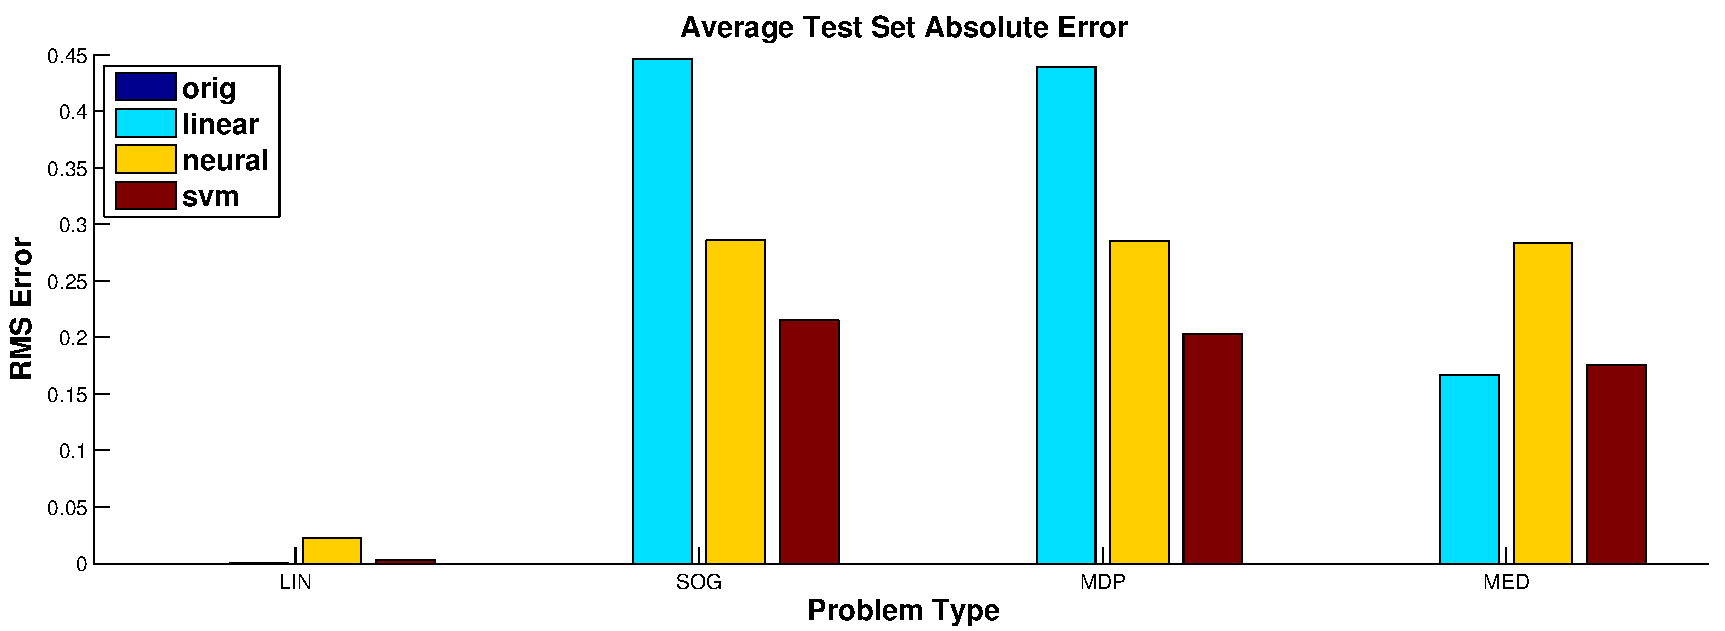
\includegraphics[width=7in]{images/results_rmse}
  \caption{TODO: System Diagram}
\end{figure}

We've implemented a compilation framework in python. Approximators derived from a base class specify how to generate a C file with an approximate version of the original function. In general, these approximators are machine learning models whose parameters are learned by training on various input/output examples. The parameter values that minimize error are incorporated into the approximate C code. That approximation code is then run from python and compared with the original.

\subsection{Approximators}

\subsubsection{Linear regression}

This approximates the original function by defining the function output to be a linear combination of the features of the input. The approximation is learned using scikit-learn's linear model package. The weights and the simple code that evaluates the linear function using those weights are what is written to file.

\subsubsection{Neural networks}

Similar to \cite{Esmaeilzadeh12}, we used a neural network to approximate functions. They were learned using a python implementation of FANN. FANN was used in the implementation of the approximation C code as well. % Danny: add any other notes here about what kind neural network we learned or whatnot

\subsubsection{SVM}

%TBA by Danny.

\section{Evaluation}

\subsection{Input Functions}

Our project was originally intended to be tested against inputs from a RoboCup planner agent, which would involve evaluating the utility of passing the ball to certain locations on the play field given the current location of robots. However, it became apparent that it would be be feasible neither to support the complex C++ function calls used in that code base nor to isolate an interesting problem that could be expressed independently of the main RoboCup code.

Instead, we evaluated several other problem domains which stand in for typical problems that face a robotic agent. Each of the problems accepts a vector of input values and outputs a two-dimensional grid of values. The size of the input vector and output grid must be fixed when generating an approximator.

\begin{itemize}
\item \textbf{Linear (LIN)} A basic problem type where each output grid value is a linear combination of the its grid coordinates. That is, the output value at grid location $(x, y)$ is $v = \alpha x + \beta y$, where the linear coefficients $\alpha$ and $\beta$ are constant over the whole grid.

\item \textbf{Sum of Gaussians (SOG)} The output of a function of this type is the sum of one or more Gaussian basis functions placed randomly on the grid. While calculating this function is rapid in quite rapid even without approximation, the terrain that it generates presents a good challenges for approximators, as it is non-linear in the function inputs.

\item \textbf{Markov decision process (MDP)} The output of problems of this type is the solution to value iteration for a Markov decision process problem instance defined over the squares of the grid, emulating the planning of a robotic agent. The agent's state is a grid position $(x, y)$ and it may move deterministically in the four cardinal directions. One or more states are assigned a randomized reward value in the range $[0, 1]$. The computation cost of value iteration scales quickly for discount factors near unity and large grid state spaces, but it permits some imprecision in the computed values per state, as long as topological features of the output are preserved. This makes it a prime candidate domain for approximation.

\item \textbf{Median filter (MED)} A median filter is used in imaging processing applications to remove noisy pixels; however, performance degrades quickly for large filter window sizes. This function applies a median filter to a 2D input image with a filter window size of $7 \times 7$ pixels. While \cite{Esmaeilzadeh12} tested image filter approximations only at the per-pixel level, our approximators operate on pairs of two-dimensional input and output image patches (in order to make keep the dimensionality of the approximation tractable, we limit the input/output images to size $20 \times 20$).
\end{itemize}

\subsection{Metrics}

\subsubsection{Error Metrics}
We use these metrics to assess how close/good our approximations are.

\begin{itemize}
\item Root mean squared error (RMSE)
\item Preservation of max and min locations (TODO: this might be changed to the gradient RMSE... TBD)
\item Qualitative (see figures)
\end{itemize}

\subsubsection{Performance Metrics}
\begin{itemize}
\item Training time - how long it took to train approximator
\item Execution time - time spent running function on inputs
\item Instruction read counts - number of instructions executed (collected using valgrind's callgrind tool)
\end{itemize}

\section{Results}

For each of the LIN, SOG, and MDP problem types, the approximators were trained on a set of 50 function input/output pairs and their quality was evaluated on a separate set of 50 test pairs. The output grids were of size $30 \times 30$ for LIN, SOG and MDP problem domains and size $20 \times 20$for the MED problem (the image chunk size).


% Tables! Graphs! Pictures!

\begin{figure}
  \centering
  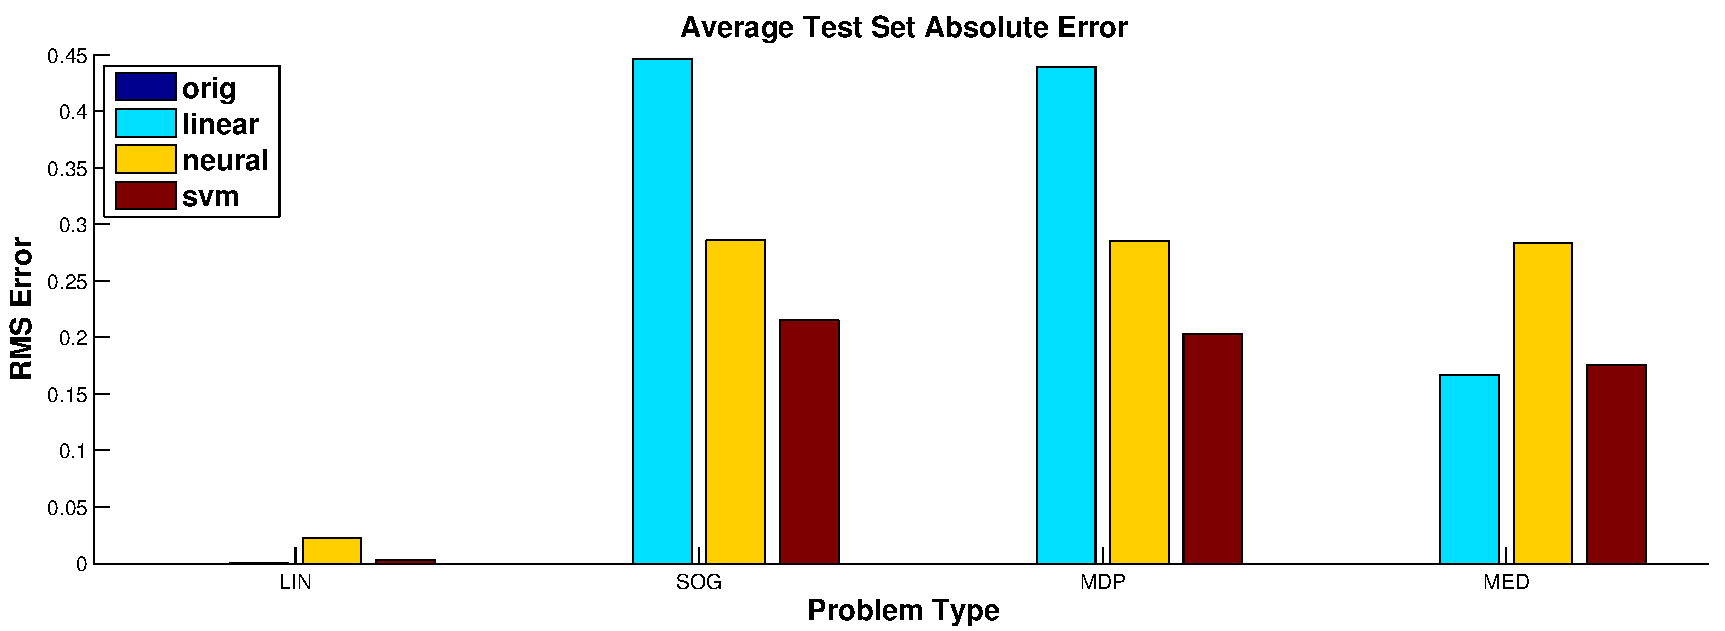
\includegraphics[width=0.8\textwidth]{images/results_rmse}
  \caption{Average test error values by approximation strategy on each of our input function domains.}
\end{figure}

\begin{figure}
  \centering
  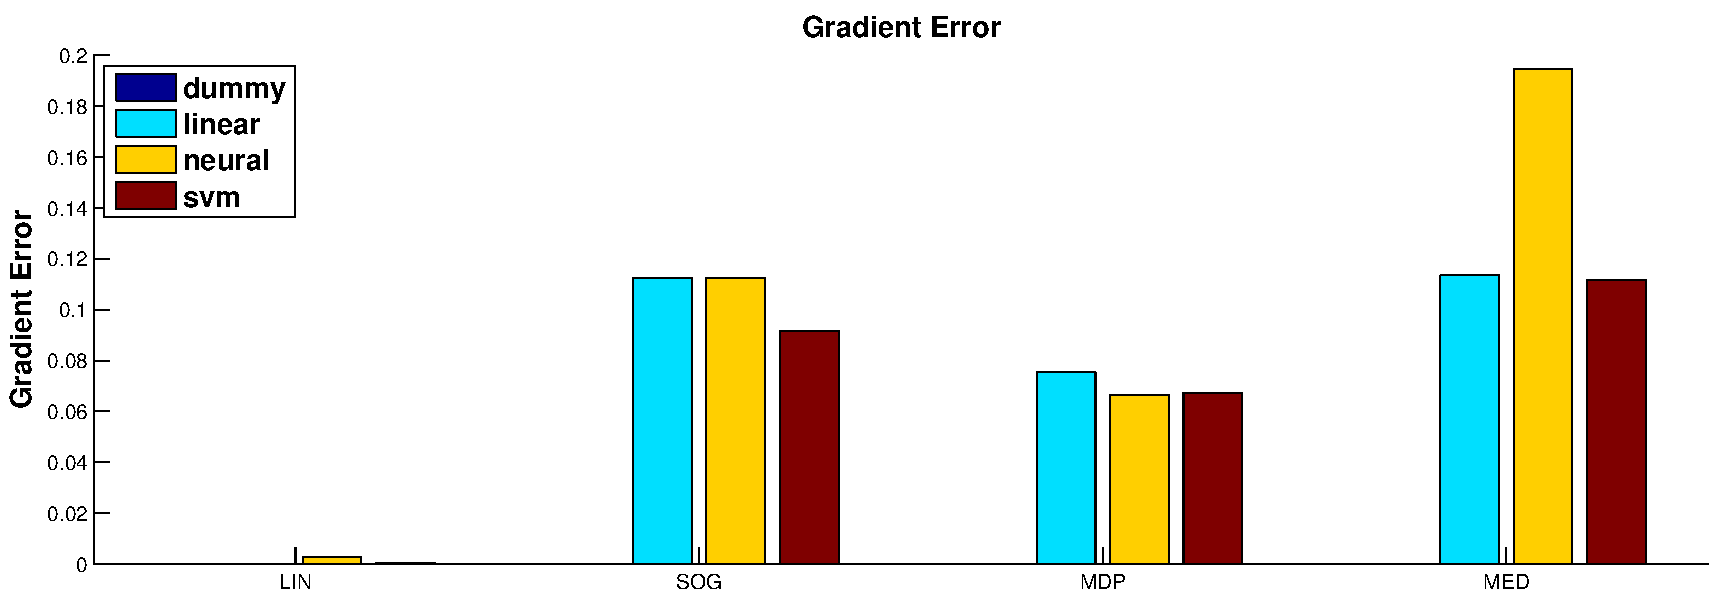
\includegraphics[width=0.8\textwidth]{images/results_grad_rmse}
  \caption{Average error of the 2D gradient over the output grid by approximation strategy . Maintaining the gradient of the original function is desirable in order to preserver the local topology of the original function output.}
\end{figure}

\begin{figure}
  \centering
  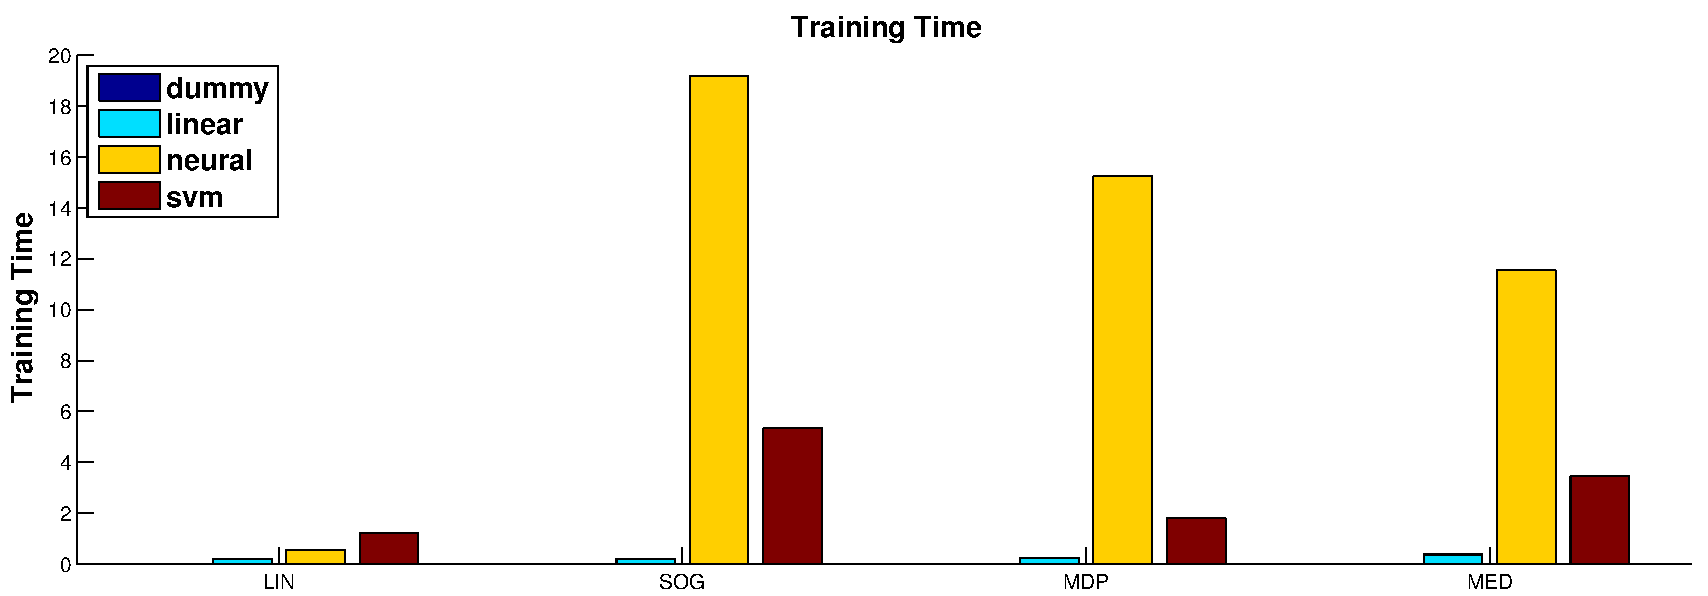
\includegraphics[width=0.8\textwidth]{images/results_run_time}
  \caption{Average function runtime by approximation strategy.}
\end{figure}

\begin{figure}
  \centering
  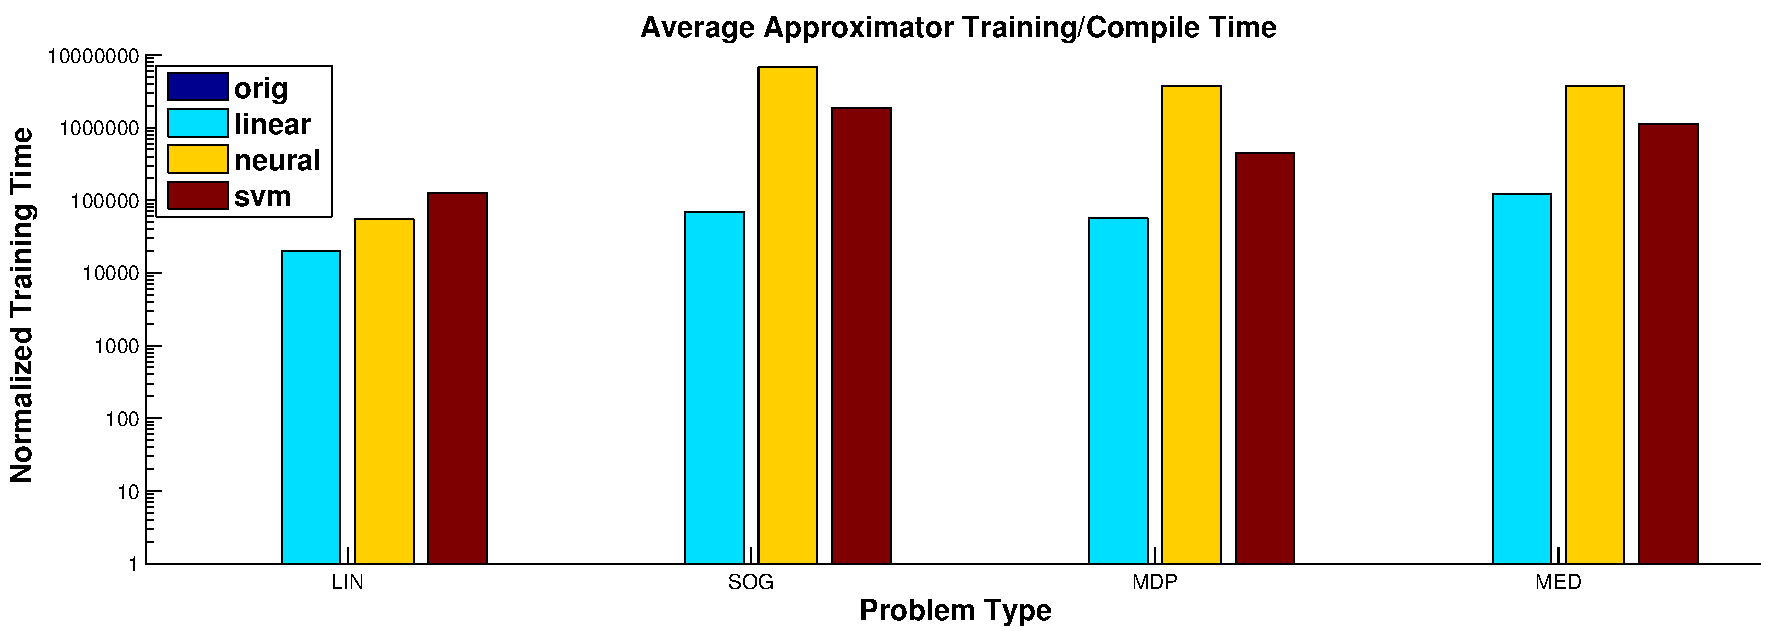
\includegraphics[width=0.8\textwidth]{images/results_train_time}
  \caption{Average test error values by approximation strategy on each of our input function domains.}
\end{figure}

\begin{figure}
  \centering
  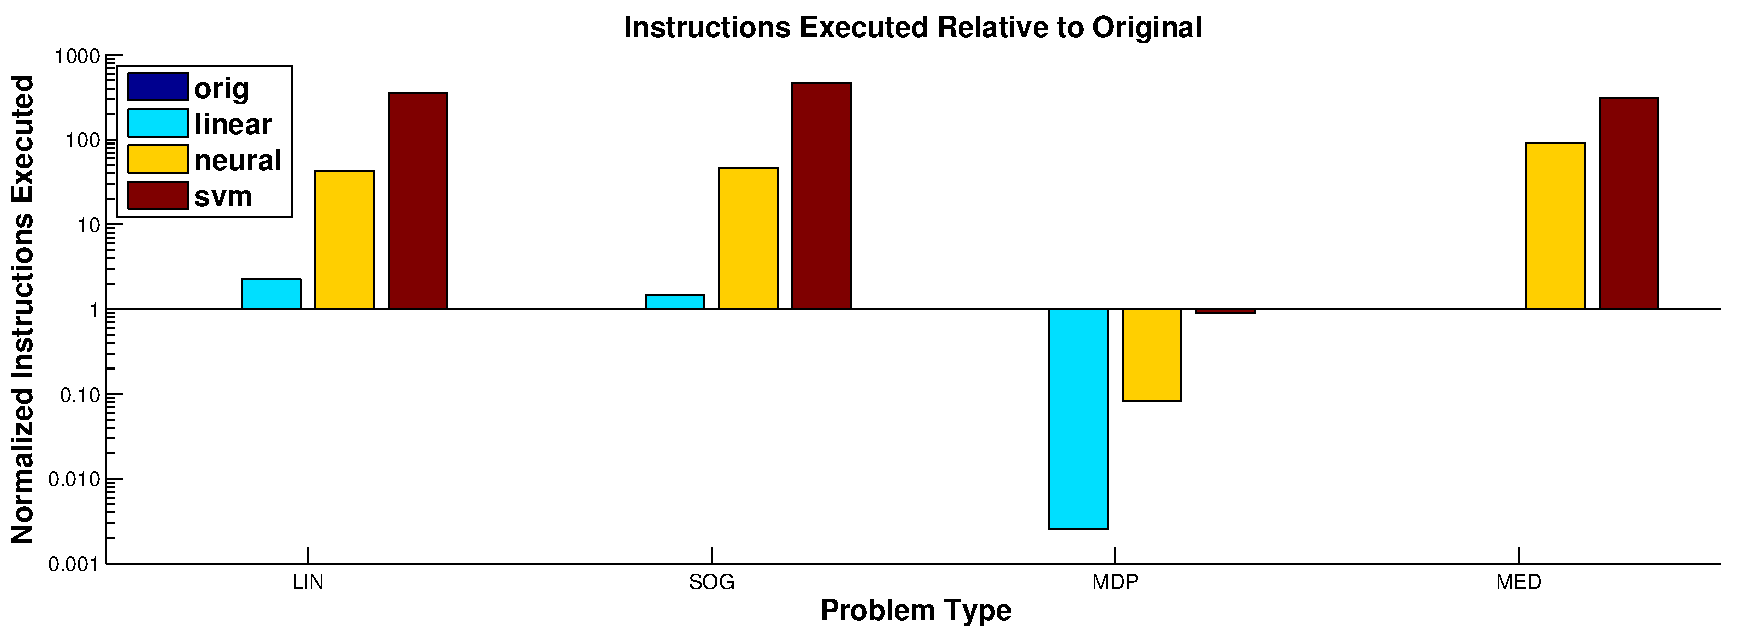
\includegraphics[width=0.8\textwidth]{images/results_instructions}
  \caption{Average number of instructions executed by approximation strategy on each of our input function domains.}
\end{figure}

\section{Discussion}

\section{Project Notes}

\bibliographystyle{ieeetr}
\bibliography{sources}

\end{document}
